\section{Main theorem: proof sketch}\label{sub:main_thm_proof_sketch} % (fold)

We have a couple of technicalities to dispatch. To motivate the
first of these we wish to note that the arguments for the
forward direction require some care. The aim is to capture the
intuitive equivalence-preserving nature of the Reidemeister moves as
corresponding bisimularity-preserving transformations on processes (in
the image of the encoding). Because of the encoding of crossing
information of wires in terms of synchronization of signal-flow, we
have to introduce ``enough signal'' to keep the knot ``firing'', as it
were, to establish that the process transformations corresponding
to the knot transformations are bisimulation-preserving. Rather than
seeing this extra condition as a weakness of the approach we submit that this feature
provides evidence to our claim that the characterization of ambient isotopy of knots at
work in this encoding is in terms of process dynamics.

We will say that the encoding of a knot is \emph{alive} as long as it
is firing, i.e. the process is enabled to make a reduction step. If it
ever ceases to push signal through, i.e. process cannot make a
reduction step, then it is \emph{dead}.
  
We can ascertain an upperbound on initial signal that guarantees
liveness of the encoding. Surely, the parallel composition of $2\#(K)$
barbs, i.e. two barbs for each crossing, will guarantee the liveness
of the encoding. More declaratively, we simply demand that $
\meaningof{K} | initSignal$ be live before we are willing to admit
it as a representation of the knot.

\begin{definition}
  More precisely, we will call the pair
  $(\meaningof{K},initSignal)$ \emph{alive} if $initSignal$ is
  an abstraction over a parallel composition of barbs, with
  $|initSignal| = |\meaningof{K}|$, we demand that for any vector
  of distinct names, $v$ with $|v| = |\meaningof{K}|$ and any state,
  $K'$, such that $\meaningof{K}\langle v \rangle | initSignal
  \langle v \rangle \wred K'$ we have that $K' \red$.
\end{definition}

\paragraph*{Different crossing numbers mean different numbers of free
  names.}
Knots in the same isotopy class may have diagrams with different numbers of
crossings. Different numbers of crossings lead to different arities
in the abstractions, so in interpreting these knots we haveto work to properly capture the notion of equivalence. While the precise statement
is somewhat technical, the intuition is simple: it is possible to find
a common ``interface'', i.e. argument list, between the two knots such
that restricting to that argument list obtains bisimilar processes.

Imagine (the processes that interpret) knots as programs housed in
boxes with ports on the perimeter. Two knot diagrams $K_i, i \in \{1,2\}$, from
the same isotopy class may have different crossing numbers and thus
their boxes have different numbers $\#(K_i)$ of ports on the outside. We can find a number of ports, call it $n$, somewhere
between the minimal crossing number of the isotopy class and the
lesser of $\#(K_i)$ such that if -- using restriction -- we close off
$\#(K_1) - n$ ports on the first box and $\#(K_2) - n$ on the second
we get two boxes that perform the same observable set of signal
processing steps.

Formally, suppose $K_{1} \sim K_{2}$ and let $\#_{Min}(K) :=
min\{\#(K') : K' \sim K \}$. We assert that there is an $n$ such that   
$4\#_{Min}(K_1) \leq n \leq 4*min\{ \#(K_1), \#(K_2) \}$ and for
any vector of names, $\vec{v}$, with $|\vec{v}| = n$ and $v[i] \neq
v[j] \iff i \neq j $, there exists two vectors of names, $\vec{w_1},
\vec{w_2}$, also all distinct, such that
\begin{eqnarray}
    (\nu \; \vec{w_1})\meaningof{K_{1}}\langle \vec{v}:\vec{w_1} \rangle & \simeq & (\nu \; \vec{w_2})\meaningof{K_{2}}\langle \vec{v}:\vec{w_2} \rangle \nonumber
  \end{eqnarray}
  with $|\vec{w_i}| = 4\#(K_{i}) - n$.

  \paragraph{Prime versus composite knots.} Finally, we need to say a
  little about how we obtain a $\pi$-calculus expression for a given
  knot diagram. We use another bootstrapping procedure, beginning with another
  knot notation (Dowker-Thistlethwaite codes is used here) and
  exhibiting an algorithm for calculating a process expression from the chosen notation scheme. The reader will
  note that DT codes are  unique only when restricted to the class of prime knots. It turns out
  that our encoding preserves knot composition. In fact, knot
  composition turns out to be a specialized form of a procedure,
  parallel composition + hiding, long-investigated in the
  process-algebraic setting. So, it is sufficient to demonstrate the
  encoding for prime knots.

\subsection{Forward direction. $ K_1 \sim K_2  \implies  \meaningof{K_1} \simeq \meaningof{K_2}$}

\paragraph*{Strategy and intuitions.} Since $K_1 \sim K_2$ we know
there is a sequence of Reidemeister moves converting $K_1$ to 
$K_2$. Each move is proved to correspond to a bisimilarity-preserving
transformation on a related process. We establish context and
substitution lemmas and as a consequence obtain that the process operations
corresponding to the Reidemeister moves preserve bisimularity. As
noted above, a small amount of bookkeeping is required to iteratively
apply these transformations to mirror Reidemeister moves as applied in a
proof of ambient isotopy of two knots.

We begin by observing that the intuition behind the Reidmeister moves
is fundamentally about performing local operations, i.e. on
some subset of wires or crossings, while leaving the rest of the
process unchanged. We interpret this notion of a ``local operation'',
say $R$, on a knot diagram $K$ schematically as follows.

\begin{itemize}
\item factor the process, $\meaningof{K}$, as $M[\Pi_iC_i | \Pi_jW_j]$
  where $\Pi_iC_i | \Pi_iW_i$ encodes the set of crossings or wires
  to be modified by $R$, i.e. the left side of the move to be
  performed, and $M$ is the context representing the unchanged portion of the process;
\item letting $R^{\to}(K)$ (resp. $R^{\leftarrow}(K)$) denote the
  left-to-right (resp. right-to-left) application of the move R to
  $K$, then $\meaningof{R^{\to}(K)}$ is calculated as
  $M[\Pi_{i'}C_{i'}' | \Pi_{j'}W_{j'}]$, where $\Pi_{i'}C_{i'}' |
  \Pi_{j'}W_{j'}$ are the processes interpreting the modified set of
  crossings or wires, i.e. the right side of the move to be performed.
\end{itemize}

The mathematical content of these statements is that the encoding
naturally extends to an encoding $\meaningof{R_{i}\{L,R\}}$ of the left and right hand sides of each
Reidemeister move such that $\meaningof{K} =
M[\meaningof{R_{i}L}]$ (resp. $M[\meaningof{R_{i}R}]$) and
$\meaningof{R_{i}^{\to}(K)} = M[\meaningof{R_{i}R}]$
(resp. $\meaningof{R_{i}^{\leftarrow}(K)} = M[\meaningof{R_{i}L}]$). Here, a picture really is worth a thousand words (see figure
\ref{fig:RMovesAsXforms}).  

\begin{example} For example,  as in
  \ref{example:trefoilcontext} taking $M_{3_1}$ to be  the encoding of $R_1(3_1,W(v_3,v_6))$,
  the application of $R_1$ to $3_1$ at to the strand corresponding to
  the wire process $W(v_3,v_6)$ is given by
  $\meaningof{R_1(3_1,W(v_3,v_6))} = (\nu \; x_{0} \; x_{1} \; y_{0}
  \; y_{1})M_{3_1}[((\nu \; u)C(x_{0},x_{1},y_{0},y_{1},u) |
  W(x_{0},x_{1}) | W(y_{0},v_{3}) | W(y_{1},v_{6}))]$. See figure
  \ref{fig:TrefoilContextIllustration}.
  
  \begin{figure}[tbp]
    \centering
    \scalebox{0.30}[0.300]{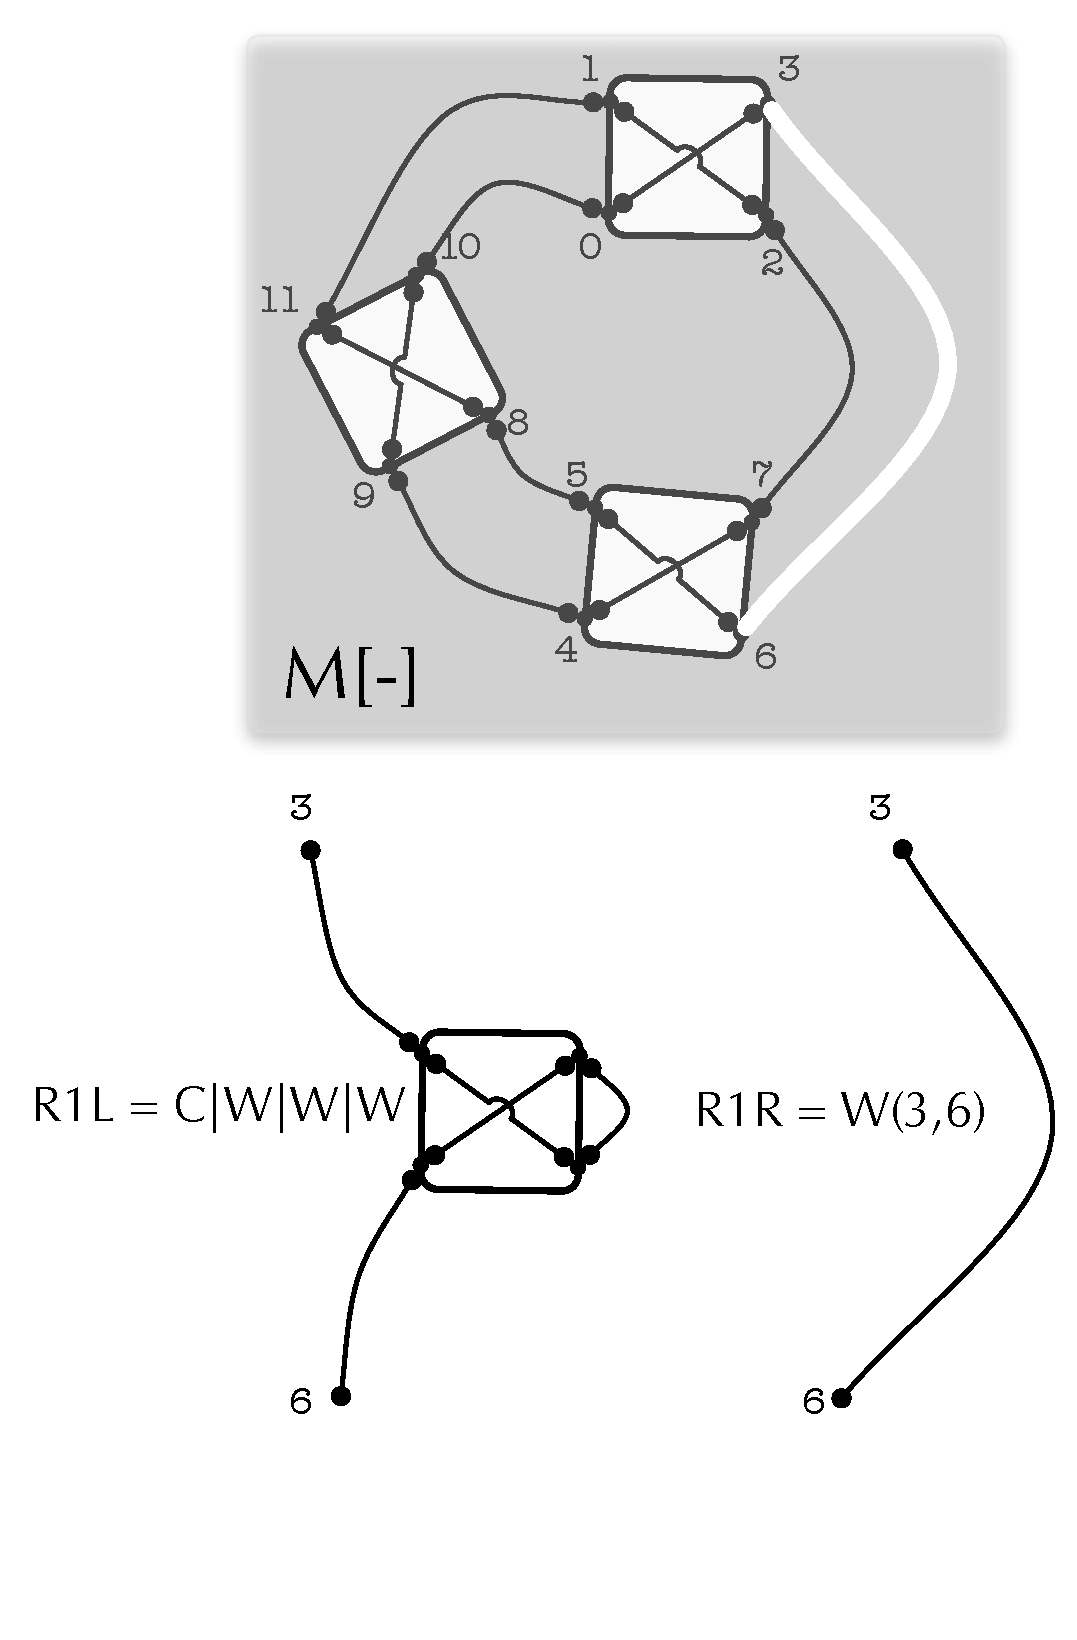
\includegraphics[viewport=30 30 810 550]{../../illustrations/TrefoilContextIllustration}}
    \caption{The figure illustrates a Reidemeister move of the first type as reflected in the context $M$ of the $3_1$  knot, as given in Ex. \ref{example:trefoilcontext}. }
  \label{fig:TrefoilContextIllustration}
\end{figure}
  % The interface of the $R_1$ move is ...
\end{example}

A certain discipline is required in the extended encoding. To
establish our substitution and context lemmas we have to keep the
\textit{interface} (\emph{i.e.} the ports in the process expression
corresponding to the splice points) of the left and right hand sides
of the R-move the same. So, for $R_{1}L$ and $R_{2}L$ we must restrict the ports
that are not the splice points. One way to address this is to embed
the restrictions into the encodings of $R_{1}L$ and $R_{2}L$. Algebraically,

  % \begin{eqnarray}
%     \lefteqn{\meaningof{R_{1}L}(y0,y1) =} \nonumber \\
%     & & (\nu \; x_{0} \; x_{1} \; v_{0} \; v_{1} ) ((\nu \; u)C(x_{0},x_{1},v_{0},v_{1},u) | W(x_{0},x_{1}) | W(y_{0},v_{0}) | W(y_{0},v_{1})) \nonumber \\
%     \lefteqn{\meaningof{R_{2}L}(x_{00},x_{01},x_{10},x_{11}) =} \nonumber \\
%     & & (\nu \; y_{00},y_{01},y_{10},y_{11},)((\nu \; u_{0})C(x_{00},x_{01},y_{00},y_{01},u{0}) \nonumber \\
%     & & | W(y_{00},y_{11}) | W(y_{01},y_{10}) | (\nu \; u_{1})C(x_{10},x_{11},y_{10},y_{11},u_1)) \nonumber
%   \end{eqnarray}

\begin{align*}
  \meaningof{R_{1}L}(y0,y1) = & \\
  (\nu \; x_{0} \; x_{1} \; w_{0} \; w_{1} ) & (W(y_{0},w_{0}) \\
  & |(\nu \; u)C(x_{0},x_{1},w_{0},w_{1},u) | W(x_{0},x_{1}) \\
  & | W(y_{1},w_{1})) \\
  \meaningof{R_{2}L}(x_{00},x_{01},x_{10},x_{11}) = & \\
  (\nu \; y_{00},y_{01},y_{10},y_{11},w_{00},w_{01},w_{10},w_{11}) & (W(x_{00},w_{00}) | W(x_{01},w_{01}) \\
  & | (\nu \; u_{0})C(w_{00},w_{01},y_{00},y_{01},u{0}) \\
  & | W(y_{00},y_{11}) | W(y_{01},y_{10}) \\
  & | (\nu \; u_{1})C(w_{10},w_{11},y_{10},y_{11},u_1) \\
  & | W(x_{10},w_{10}) | W(x_{11},w_{11}))
\end{align*}

  Keeping to the notion of equivalence outlined in the section above,
  however, it will be convenient to factor out the restrictions as in
  the example above.

\begin{figure}[tbp]
%  \centering
 % \scalebox{0.35}[0.350]{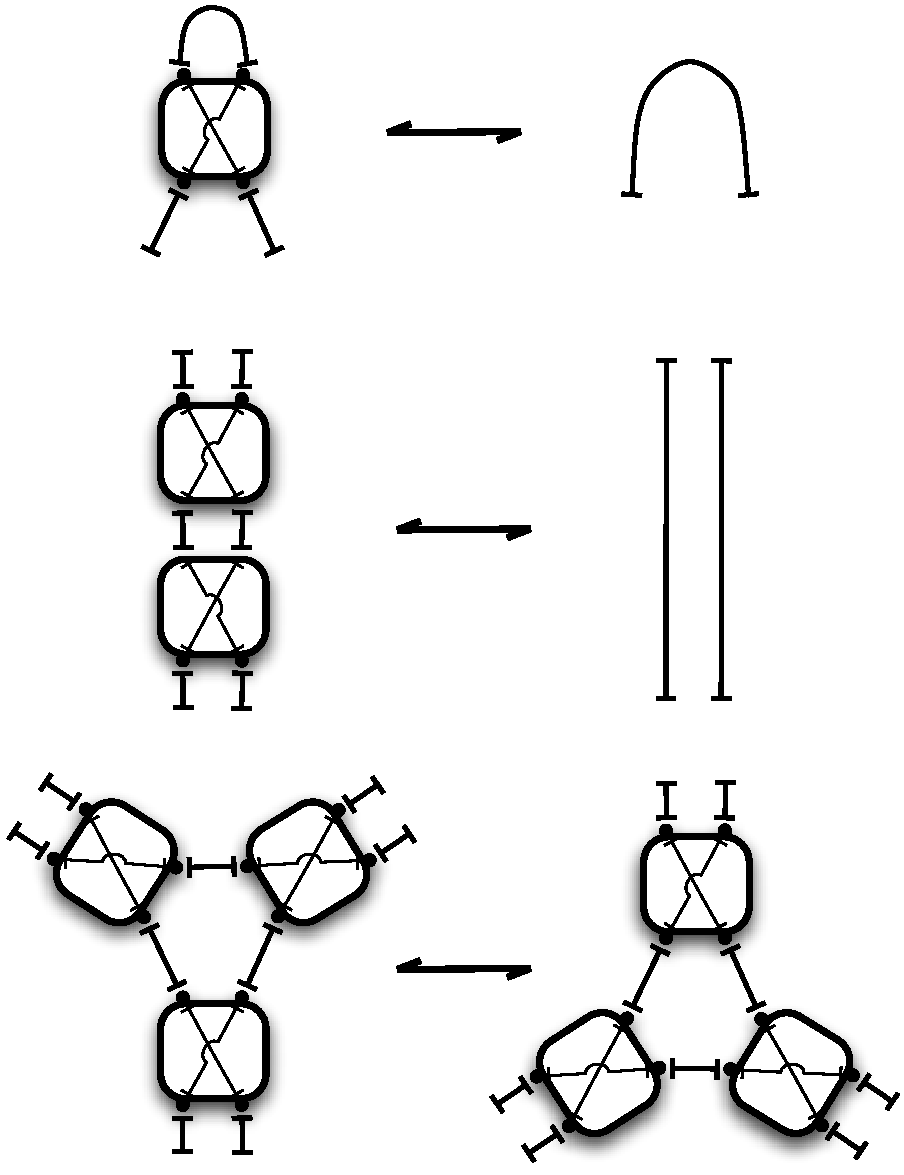
\includegraphics[viewport=30 30 810 550]{../../illustrations/ReidemeisterMovesAsCircuits071115.pdf}}
% Reidemeistermovesascircuits21072006

\center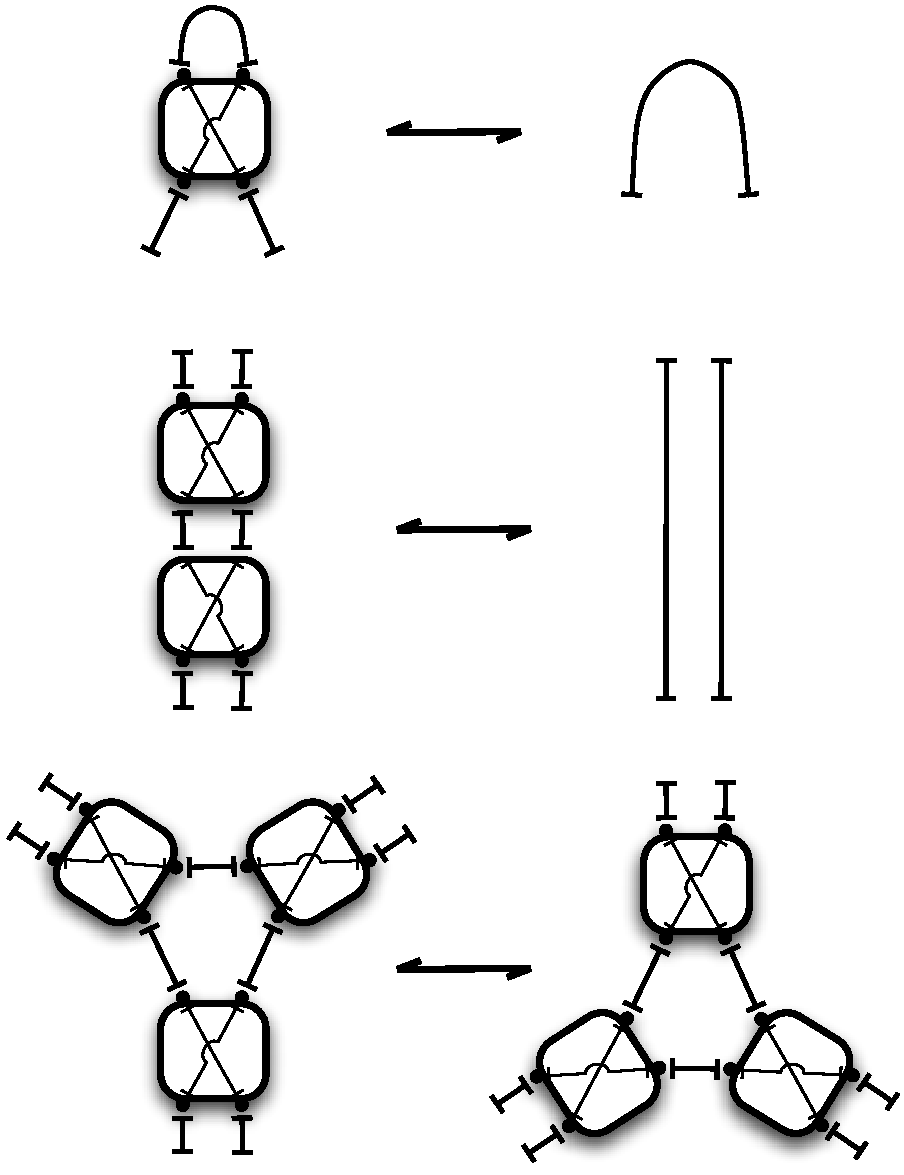
\includegraphics[width=3in]{../../illustrations/ReidemeisterMovesAsCircuits071115.pdf}  
\caption{ Reidemeister moves as bisimilarity-preserving transformations. Cf. Fig. \ref{fig:RMoves}}

\label{fig:RMovesAsXforms}
\end{figure}

\begin{lemma}[context]
$\forall i \in \{ 1, 2, 3 \}$ if $K_{1} \stackrel{R_{i}}{\rightarrow}
K_{2}$ then there exists a context $M$ and (possibly empty) vector of
distinct names $\vec{w}$ such that
  \begin{eqnarray}
    (\nu \; \vec{w})\meaningof{K_{1}}\langle v:w\rangle & = & (\nu \; \vec{w})M[ \meaningof{R_{i}L} ] \nonumber \\
    \meaningof{K_{2}} & = & M[ \meaningof{R_{i}R} ] \nonumber
  \end{eqnarray}
\label{context}
\end{lemma}

\begin{proof}
  This follows directly from the definition of the encoding.
\end{proof}

\begin{lemma}[substitution]
  For all $i \in \{ 1, 2, 3 \}$ $R_{i}L$ is bisimilar to $R_{i}R$ in the
  context of a live encoding. That is, if
  \begin{itemize}
    \item $\meaningof{K} | initSignal$ is alive, and
    \item $\meaningof{K} | initSignal = M[ \meaningof{R_{i}L} ]$
  \end{itemize}
for some context $M$ then we can substitute $\meaningof{R_{i}R}$ in
  its place without change of behavior, i.e.
  \begin{eqnarray}
    (\nu \; \vec{w})M[ \meaningof{R_{i}L} ] & \simeq & M[ \meaningof{R_{i}R} ] \; ,\ \forall i \in \{ 1, 2, 3 \} \nonumber
  \end{eqnarray}
\end{lemma}

\begin{proof}
  This follows from the definitions of $\meaningof{R_{i}\{L,R\}}$ plus
  the requirement that $M$ derives from a live encoding. Even if one
  side has additional synchronizations, there is always enough signal
  to overcome spurious blocking.
\end{proof}

An immediate consequence of these two lemmas is 

\begin{lemma}[1-step]
  if $K_{1}$ can be derived from $K_{2}$ by application of one Reidemeister move, then 

  \begin{eqnarray}
    \meaningof{K_{1}}\langle v \rangle & \simeq & (\nu \; w)\meaningof{K_{2}}\langle v:w \rangle \nonumber
  \end{eqnarray}
\end{lemma}

We are almost in a position to complete the proof of the forward
implication. The next step is to show that you can iterate the
performance of these bisimilarity-preserving transformations in a way
that precisely mimics iterated application of Reidemeister
moves. Because the moves $R_{1}$ and $R_{2}$ change the number of
crossings the number of ports in the interface of the (encoding of
the) knot to which they are applied changes. This is the core issue in
the formal statement of the theorem. Because the splice interface
remains constant across the two sides of a Reidemeister move all one
has to do is keep track of the ports to be hidden. The complete proof
uses a case analysis of the composition of any two types of
Reidemeister moves. We illustrate the analysis in the case of a
simplifying (crossing-elimination) $R_1$ step followed by a complicating
(crossing-introducing) $R_2$ step.

\begin{itemize}
   \item The $R_{1}L$ $\to$ $R_{1}R$ step means we have a context $M$ such that
     \begin{eqnarray}
       (\nu \; x_0 \; x_1 \; w_0 \; w_1)\lefteqn{\meaningof{K_{1}}\langle \vec{v_0}:x_0 : x_1 : w_0 : w_1\rangle} \nonumber \\
       & & = (\nu \; x_0 \; x_1 \; w_0 \; w_1)M[ \meaningof{R_{1}L} ] \nonumber \\
       & & \simeq M[ \meaningof{R_{1}R} ] \nonumber \\
       & & = \meaningof{K_{2}}\langle \vec{v_0} \rangle. \nonumber
     \end{eqnarray}
   \end{itemize}

   \begin{itemize}
   \item The  $R_{2}R$ $\to$ $R_{2}L$ step means we have a context $M'$ such that
     \begin{eqnarray}
       (\nu \; y_{00} \ldots y_{11} \; w_{00} \ldots w_{11})\lefteqn{\meaningof{K_{3}}\langle \vec{v_1}:y_{00}:\ldots : y_{11} : w_{00} : \ldots : w_{11} \rangle} \nonumber \\
       & & = (\nu \; y_{00} \ldots y_{11} \; w_{00} \ldots w_{11})M'[ \meaningof{R_{2}L} ] \nonumber \\
       & & \simeq M'[ \meaningof{R_{1}R} ] \nonumber \\
       & & = \meaningof{K_{2}}\langle \vec{v_1} \rangle. \nonumber
     \end{eqnarray}
   \end{itemize}

\begin{itemize}
     \item Since $\vec{v_0}, \vec{v_1}$ are just lists of distinct names with
      $|\vec{v_0}| = |\meaningof{K_{2}}| = |\vec{v_1}|$, just pick $\vec{v_0} = \vec{v_1}$. Dropping the subscript, we conclude 
     \begin{eqnarray}
       \lefteqn{(\nu \; x_0 \; x_1 \; w_0 \; w_1)\meaningof{K_{1}}\langle \vec{v}:x_0 : x_1 : w_0 : w_1 \rangle \simeq} \nonumber \\
       & & (\nu \; y_{00} \ldots y_{11} \; w_{00} \ldots w_{11})\meaningof{K_{3}}\langle \vec{v_1}:y_{00}:\ldots : y_{11} : w_{00} : \ldots : w_{11} \rangle \nonumber
     \end{eqnarray}
     \item Moreover, we have  $\meaningof{K_{2}}\langle \vec{v} \rangle$ forming the shared core.
   % \item hence $x_0,x_1$ do not occur free in $\vec{v}:y_{00} : y_{01} : y_{10} : y_{11}$,
%      and $y_{00}, y_{01}, y_{10}, y_{11}$ do not occur free in $\vec{v}:x_0 : x_1$
%    \item applying scope extrusion, twice, therefore yields the desired result.
   \end{itemize}

\subsection{Reverse direction. $ K_1 \sim K_2  \Leftarrow  \meaningof{K_1} \simeq \meaningof{K_2}$}

We prove this by contradiction,
assuming two knots in distinct isotopy classes with bisimilar images
and arriving at absurdity. Not surprisingly, the argument in this
direction is considerably less complicated as it is nonconstructive.

Without loss of generality (by application of the lemmas of the forward direction as needed), we assume knots are given in minimal
crossing diagrams. Due to this minimality, if the crossing
numbers of these diagrams are different, then the number of free names (or arity of the
abstractions interpreting the knots)  in  $\meaningof{K_1}$  differs from those  in $\meaningof{K_2}$ --contradicting
bisimilarity. Thus, the crossing numbers must be the same. 

Now we employ the form of the encoding: $\Pi_{i=0}^{n-1}
\meaningof{C(i)}(...) | \Pi_{i=0}^{n-1} W(...)|W(...) \simeq
\Pi_{j=0}^{n-1} \meaningof{C(j)}(...) | \Pi_{j=0}^{n-1}
W'(...)|W'(...)$. Notice that a consequence of sharing the same
crossing number is that the crossing process part of the two encodings
is \emph{identical}. Because bisimulation is a congruence this implies
$\Pi_{i=0}^{n-1} W(...)|W(...) \simeq \Pi_{j=0}^{n-1}
W'(...)|W'(...)$. This says that the only difference can be in the
``wiring harnesses''. Obviously, if any of these wires differ (up to $\alpha$-equivalence), then there
is a  distinguishing barb, contradicting our assumption of
bisimulation.  Hence none of the wires differ, their respective sets of crossings are wired
identically, which means the diagrams are identical. Thus, the knots are ambiently isotopic -- a contradiction.

%\subsection{Strengthening the statement of the theorem}
%
%Let
%  
%   \begin{eqnarray}
%     \lefteqn{L_C(\meaningof{K}\langle \vec{u} \rangle, \vec{v}) :=} \nonumber \\
%     & & \{ (\nu \; u)C(\vec{z}) : \exists P \; \meaningof{K}\langle \vec{u} \rangle = (\nu \; u)C(\vec{z}) | P \} \nonumber \\
%     \lefteqn{L_W(\meaningof{K}\langle \vec{u} \rangle, \vec{v}, \vec{w}) :=} \nonumber \\
%     & & \{ W(a,b) : \exists P \; \meaningof{K}\langle \vec{u} \rangle = W(a,b) | P, a,b \in \vec{v}, a, b \not\in \vec{w} \} \nonumber \\
%     \lefteqn{L(\meaningof{K}\langle \vec{u} \rangle, \vec{v}, \vec{w}) :=} \nonumber \\
%     & & \Pi_{C \in L_{c}(\meaningof{K}\langle \vec{u} \rangle, \vec{v})}C | \Pi_{W \in L_{W}(\meaningof{K}\langle \vec{u} \rangle, \vec{v}, \vec{w})} W \nonumber
%   \end{eqnarray}
%
%   we also have
%
%   \begin{eqnarray}
%     L(\meaningof{K_{1}}\langle \vec{v}:\vec{w_1} \rangle,\vec{v},\vec{w_1}:\vec{w_2}) = L(\meaningof{K_{2}}\langle \vec{v}:\vec{w_2} \rangle,\vec{v},\vec{w_1}:\vec{w_2}) \nonumber
%   \end{eqnarray}
%
%  \begin{itemize}
%  \item When the knots are ambient isotopic the encodings
%    \textit{share} a set of crossings and wires at least as big as a
%    minimal crossing representative of the isotopy class.
%  \item And the other parts are R-move complications of wires that
%    would complete the knot from shared core -- hidden under restriction.
%  \end{itemize}